 \documentclass[11pt,pdf,unicode,slidestop,mathserif,notes=hide,
hyperref={colorlinks=false,bookmarksopen=true,bookmarksnumbered=true,bookmarksopenlevel=1,pdfstartview={FitH},pdfborder{0 0 0}}]{beamer}
 %\usepackage[off]{auto-pst-pdf}
 \usepackage{beamerthemesplit}
\mode<transition>{
  \transblindshorizontal[duration=1]
  \transduration<1-16>{1}
}
\mode<presentation>{
  \usetheme{Copenhagen}%Antibes,Berkeley, Berlin, Copenhagen, Warsaw, Boadilla
% Remove navigation panel
  \setbeamertemplate{navigation symbols}{}
% Picture numbering
  \setbeamertemplate{caption}[numbered]
% If you wish to uncover everything in a step-wise fashion, uncomment the following command:
% \beamerdefaultoverlayspecification{<+->}
}
%% Uncomment to print
% \usepackage{pgfpages}
% \pgfpagesuselayout{4 on 1}[a4paper,border shrink=5mm,landscape]
%%\pgfpagesuselayout{resize}[a4paper,border shrink=5mm,landscape]
%\mode<handout>{
% \setbeamercolor{backgroundcanvas}{bg=black!5}
%}
 \usepackage[T2A]{fontenc}
 \usepackage[cp1251]{inputenc}
 \usepackage[english]{babel}%,russian
%% Set path for graphics
 \graphicspath{{pict/}}
%% Construct title page
 \title[Short Name]{Presentation name}
 \author[Author]{Author Name}
 \date[\today]{\today}
 \institute[CMF]{CMF MSU}
%\subject{}
 \keywords{CMF, MSU}

\begin{document}
\begin{frame}
 \titlepage
%\small{\centerline{\textcolor{blue}{add text on the titlepage}}}
\end{frame}
\setcounter{framenumber}{0}

\section[Introduction]{Introduction}
\begin{frame}{Introduction}\label{Frame:Introduction}
 \begin{itemize}%[<+-| structure@+>]
  \item Journal name
  \item Author name
  \item Main task
  \item Relevance of the work
 \end{itemize}
\end{frame}
\note{You can add some notes if you wish...}

\section[Review]{Literature review}
%2. Îáçîð ëèòåðàòóðû (êîòîðûé äåëàåò àâòîð â íà÷àëå ñòàòüè, èç íåãî äîëæíà áûòü ïîíÿòíà àêòóàëüíîñòü ðàáîòû).
\begin{frame}{Literature review}%[allowframebreaks]%\frametitle<presentation>{References}
  \begin{thebibliography}{10}
  \beamertemplatearticlebibitems
  \bibitem{Art01}
    Author
    \newblock Article name
    \newblock {\em Journal name} (2010)
  \beamertemplatearticlebibitems
  \bibitem{Art02}
    First Author and Second Author
    \newblock Article name
    \newblock {\em Journal name} (2015) (in press)
  \end{thebibliography}
\end{frame}

\section[Model]{Model/Method Description}
\begin{frame}\label{Frame:Description}
\begin{exampleblock}{Model/Method description}
\par Model description starts here
\par ...
\end{exampleblock}
\end{frame}

%4. Ýìïèðè÷åñêàÿ ÷àñòü ñ ãðàôèêàìè è òàáëèöàìè (åñëè îíè åñòü), èç íèõ äîëæíî áûòü ïîíÿòíî, êàêèå ðåçóëüòàòû ïîëó÷åíû è ÷òî ýòè ðåçóëüòàòû äîñòîâåðíû.
%5. Çàêëþ÷åíèå – êîðîòêî îñíîâíûå ðåçóëüòàòû è èõ íîâèçíà.

\section[Example]{Empirical Part of the Work}
\begin{frame}
\begin{center}
  \begin{figure}[ht]
   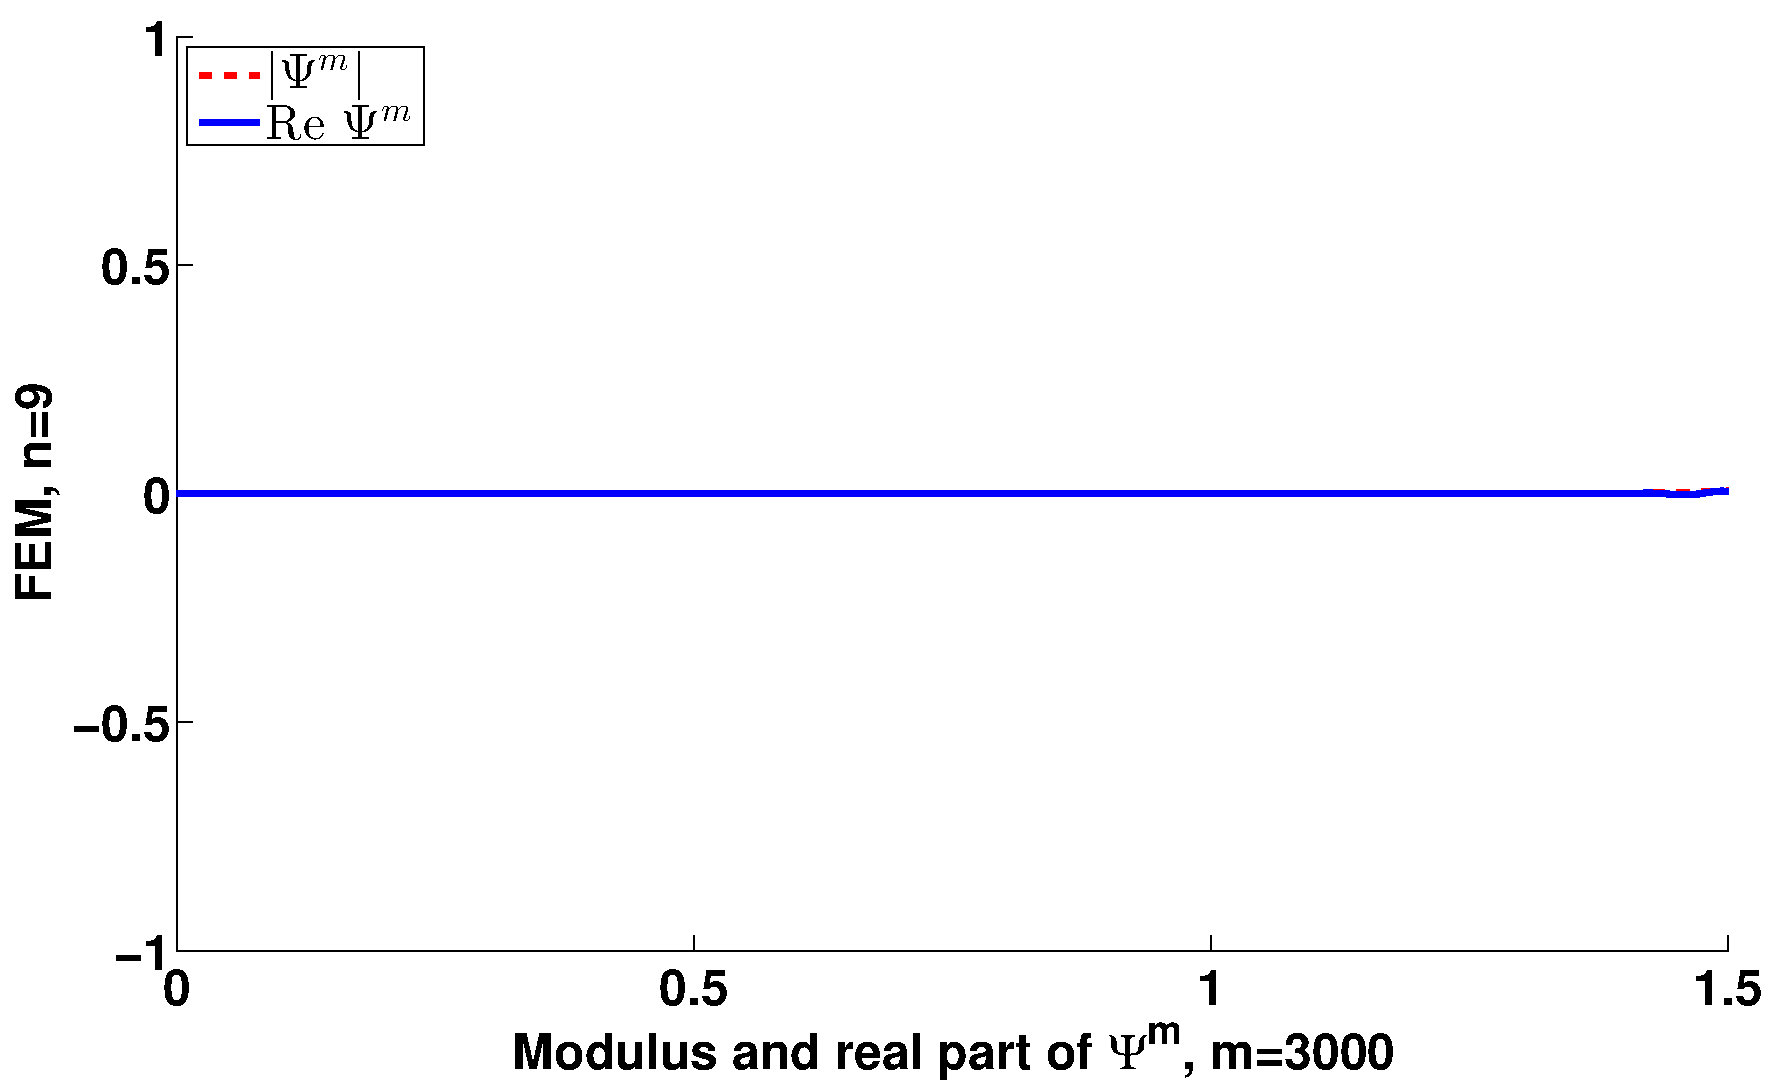
\includegraphics[width=1\linewidth]{20120309_230921_1D_EX01_SOLUTION_FEM_N=9,J=30,M=3000_k=3000_C}
   \caption{Caption name}
  \end{figure}
 \end{center}
%\vfill\hyperlink{Frame:Introduction}{\beamergotobutton{Introduction}}
%\hfill\hyperlink{Frame:Example}{\beamergotobutton{Example}}
%\hfill\hyperlink{Frame:Conclusion}{\beamergotobutton{Conclusion}}
\end{frame}

\begin{frame}\label{Frame:Picture}
 \begin{center}
  \begin{figure}[htbp]
    \begin{minipage}[h]{0.9\linewidth}
        \center{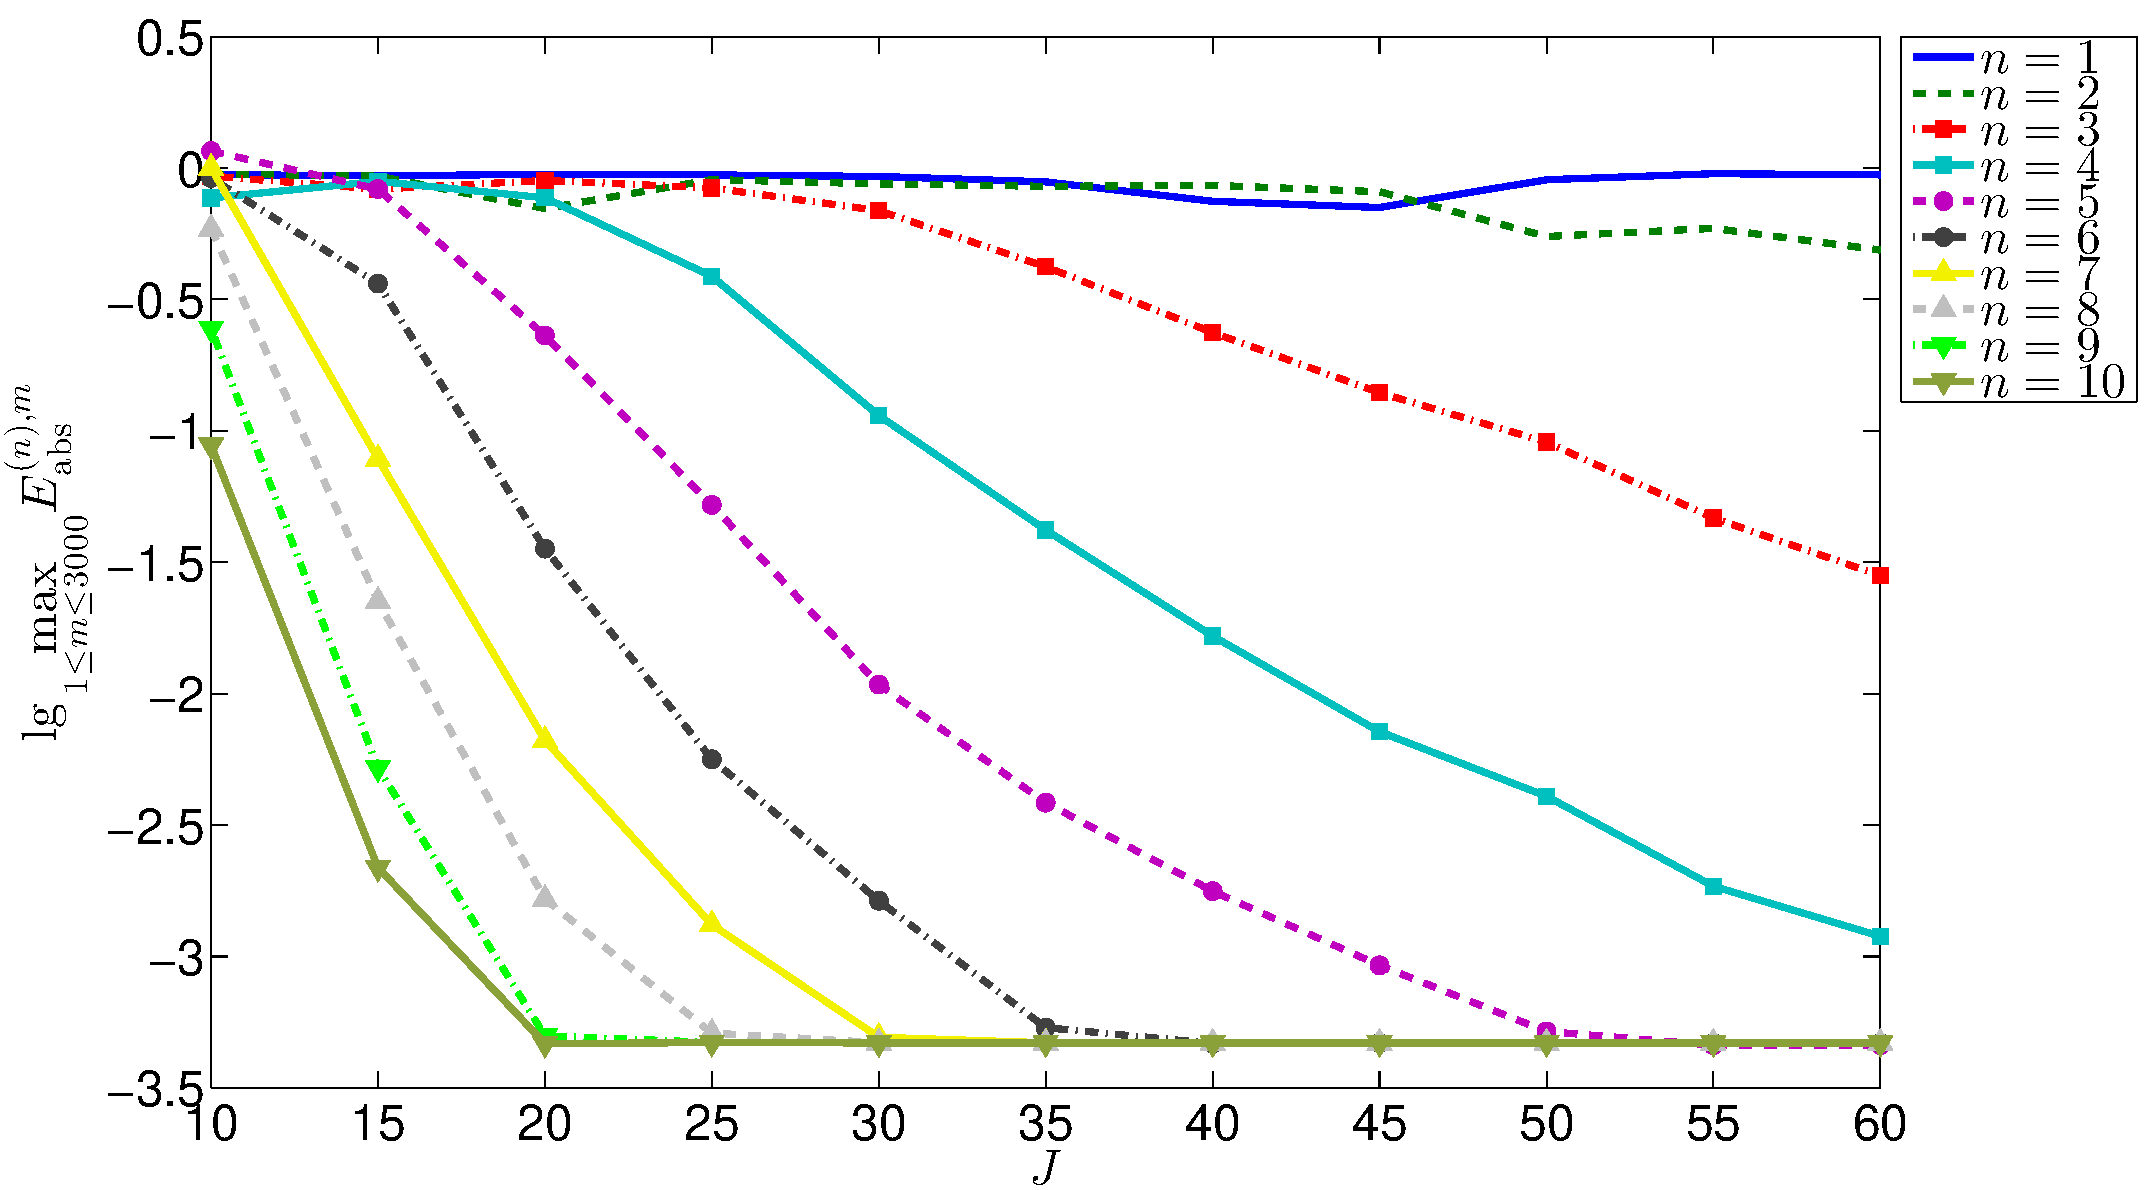
\includegraphics[width=1\linewidth]{20120314_121919_1D_EX01_MaxError_N=1,2,3,4,5,6,7,8,9,10_abs_L2_M=3000_C}}
    \end{minipage}
    \caption{\small{Another graphics description}}
    \label{fig:EX01:FEM:MaxAbsErrorL2}
  \end{figure}
 \end{center}
\vfill\hyperlink{Frame:Introduction}{\beamergotobutton{Introduction}}%\hfill
\end{frame}

\section{Conclusion}
\begin{frame}{Personal Conclusion}\label{Frame:Conclusion}
 \begin{itemize}%[<+-| structure@+>]
  \item first thesis
  \item second thesis
  \item ...
 \end{itemize}
\end{frame}
\note{You can add some notes if you wish...}

\appendix
\section<presentation>*{Additional references}
\begin{frame}{Additional references}%[allowframebreaks]%\frametitle<presentation>{References}
  \begin{thebibliography}{10}
  \beamertemplatearticlebibitems
  \bibitem{Art01}
    Author
    \newblock Article name
    \newblock {\em Journal} (2010)
  \beamertemplatebookbibitems
  \bibitem{Art02}
    First Author and Second Author
    \newblock Book name
    \newblock {\em Publisher} (2015)
  \end{thebibliography}
\end{frame}
\end{document} 